% -*- TeX -*-
\documentclass{beamer}

\usepackage{tikz}
\usetikzlibrary{shapes,arrows,calc}
\usetikzlibrary{decorations.pathreplacing}
\usetikzlibrary{fit,matrix}


\title{Crustal Deformation Modeling Tutorial}
\subtitle{PyLith and CUBIT/Trelis Refresher}
\author{Brad Aagaard \\
  Charles Williams \\
  Matthew Knepley}
\institute{
\includegraphics[scale=0.4]{../../logos/cig_blackfg}}
\date{June 23, 2014}


% ---------------------------------------------------- CUSTOMIZATION
\renewcommand{\thispdfpagelabel}[1]{}
\newcommand{\newfeature}[1]{{\color{red}#1}}
\newcommand{\status}[1]{{[\color{blue}#1]}}
\newcommand{\important}[1]{{\color{red}#1}}
\newcommand{\issue}[2]{\item[Issue:] {\color{red}#1}\\{\item[Soln:] \color{blue}#2}\\[4pt]}
\usetheme{CIG}

\newcommand{\tensor}[1]{\overline{#1}}

% ========================================================= DOCUMENT
\begin{document}

% ------------------------------------------------------------ SLIDE
\maketitle

% ------------------------------------------------------------ SLIDE
\logo{
\includegraphics[height=4.5ex]{../../logos/cig_blackfg}}

% ========================================================== SECTION
\section{PyLith}
\subsection{Overview}

% ------------------------------------------------------------ SLIDE
\begin{frame}
  \frametitle{Crustal Deformation Modeling}
  \summary{Elasticity problems where geometry does not change significantly}

  \vfill
  Quasi-static modeling associated with earthquakes
  \vfill

  \begin{itemize}
  \item Strain accumulation associated with interseismic deformation
    \begin{itemize}
    \item What is the stressing rate on faults X and Y?
    \item Where is strain accumulating in the crust?
    \end{itemize}
  \item Coseismic stress changes and fault slip
    \begin{itemize}
    \item What was the slip distribution in earthquake A?
    \item How did earthquake A change the stresses on faults X and Y?
    \end{itemize}
  \item Postseismic relaxation of the crust
    \begin{itemize}
    \item What rheology is consistent with observed postseismic deformation?
    \item Can aseismic creep or afterslip explain the deformation?
    \end{itemize}
  \end{itemize}
  \vfill

\end{frame}


% ------------------------------------------------------------ SLIDE
\begin{frame}
  \frametitle{Crustal Deformation Modeling}
  \summary{Elasticity problems where geometry does not change significantly}

  \vfill
  Dynamic modeling associated with earthquakes
  \vfill

  \begin{itemize}
  \item Modeling of strong ground motions
    \begin{itemize}
    \item Forecasting the amplitude and spatial variation in ground
      motion for scenario earthquakes
    \end{itemize}
  \item Coseismic stress changes and fault slip
    \begin{itemize}
    \item How did earthquake A change the stresses on faults X and Y?
    \end{itemize}
  \item Earthquake rupture behavior
    \begin{itemize}
    \item What fault constitutive models/parameters are consistent
      with the observed rupture propagation in earthquake A?
    \end{itemize}
  \end{itemize}
  \vfill

\end{frame}


% ------------------------------------------------------------ SLIDE
\begin{frame}
  \frametitle{Crustal Deformation Modeling}
  \summary{Elasticity problems where geometry does not change significantly}

  \vfill
  Volcanic deformation associated with magma chambers and/or dikes
  \begin{itemize}
  \item Inflation
    \begin{itemize}
    \item What is the geometry of the magma chamber?
    \item What is the potential for an eruption?
    \end{itemize}
  \item Eruption
    \begin{itemize}
    \item Where is the deformation occurring?
    \item What is the ongoing potential for an eruption?
    \end{itemize}
  \item Dike intrusions
    \begin{itemize}
    \item What is the geometry of the intrusion?
    \item What is the pressure change and/or amount of opening/dilatation?
    \end{itemize}
  \end{itemize}
  \vfill

\end{frame}


% ------------------------------------------------------------ SLIDE
\begin{frame}
  \frametitle{Crustal Deformation Modeling}
  \summary{Overview of workflow for typical research problem}

  \usetikzlibrary{arrows,shapes}
\definecolor{yellow}{rgb}{1.0, 1.0, 0.45} % 255/255/115
\definecolor{dkyellow}{rgb}{0.9, 0.9, 0.0} % % 230/230/0

\definecolor{ltorange}{rgb}{1.0, 0.74, 0.41} % 255/188/105
\definecolor{orange}{rgb}{0.96, 0.50, 0.0} % 246/127/0

\definecolor{ltred}{rgb}{1.0, 0.25, 0.25} % 255/64/64
\definecolor{red}{rgb}{0.79, 0.00, 0.01} % 201/0/3

\definecolor{ltpurple}{rgb}{0.81, 0.57, 1.00} % 206/145/255
\definecolor{purple}{rgb}{0.38, 0.00, 0.68} % 97/1/175

\definecolor{ltblue}{rgb}{0.2, 0.73, 1.0} % 51/187/255
\definecolor{blue}{rgb}{0.12, 0.43, 0.59} % 30/110/150

\definecolor{ltltgreen}{rgb}{0.7, 1.00, 0.7} % 96/204/14
\definecolor{ltgreen}{rgb}{0.37, 0.80, 0.05} % 96/204/14
\definecolor{green}{rgb}{0.23, 0.49, 0.03} % 59/125/8
  
\definecolor{dkslate}{rgb}{0.18, 0.21, 0.28} % 47/53/72
\definecolor{mdslate}{rgb}{0.45, 0.50, 0.68} % 114/127/173
\definecolor{ltslate}{rgb}{0.85, 0.88, 0.95} % 216/225/229

\tikzstyle{phase} = [rectangle, 
                      draw=dkyellow!80!black,
                      top color=yellow,
                      bottom color=dkyellow]
\tikzstyle{cig} = [rectangle, 
                      rounded corners=0.5em,
                      draw=orange!80!black,
                      top color=ltorange!50!white,
                      bottom color=orange]
\tikzstyle{open} = [rectangle, 
                      rounded corners=0.5em,
                      draw=green!80!black,
                      top color=ltgreen!20!white,
                      bottom color=green]
\tikzstyle{free} = [rectangle, 
                      rounded corners=0.5em,
                      draw=blue!80!black,
                      top color=ltblue!20!white,
                      bottom color=blue]
\tikzstyle{commercial} = [rectangle, 
                      rounded corners=0.5em,
                      draw=ltred!80!black,
                      top color=ltred!20!white,
                      bottom color=red!70!white!100]
\tikzstyle{available} = [thick, color=black]
\tikzstyle{planned} = [thick, dashed, color=mdslate]


\begin{center}
\begin{tikzpicture}[scale=0.75, transform shape,
  node distance=3.0em,
  text width=6em, text centered, minimum height=2em, thick]

  % Phases
  \node (structure) [phase] {Geologic Structure};
  \node (meshing) [phase, right of=structure, xshift=6em] {Mesh Generation};
  \node (physics) [phase, right of=meshing, xshift=6em] {Physics Code};
  \node (viz) [phase, right of=physics, xshift=6em] {Visualization};

  % Geologic structure
  \node (gocad) [commercial, below of=structure] {Gocad};
  \node (earthviz) [commercial, below of=gocad] {Earth Vision};

  % Mesh generation
  \node (cubit) [commercial, below of=meshing] {CUBIT};
  \node (lagrit) [free, below of=cubit] {LaGriT};
  \node (tetgen) [open, below of=lagrit] {TetGen};
  \node (gmsh) [open, below of=tetgen] {Gmsh};

  % Physics code
  \node (pylith) [cig, below of=physics] {PyLith};
  \node (relax) [cig, below of=pylith] {Relax};
  \node (geofest) [free, below of=relax] {GeoFEST};
  \node (abaqus) [commercial, below of=geofest] {Abaqus};

  % Visualization
  \node (paraview) [open, below of=viz] {ParaView};
  \node (visit) [open, below of=paraview] {Visit};
  \node (matlab) [commercial, below of=visit] {Matlab};
  \node (matplotlib) [open, below of=matlab] {Matplotlib};
  \node (gmt) [open, below of=matplotlib] {GMT};

  % Paths
  \path (gocad.east) edge[available] (cubit.west);
  \path (gocad.east) edge[available] (lagrit.west);
  \path (earthviz.east) edge[available] (cubit.west);
  \path (earthviz.east) edge[available] (lagrit.west);

  \path (cubit.east) edge[available] (pylith.west);
  \path (cubit.east) edge[available] (abaqus.west);
  \path (lagrit.east) edge[available] (pylith.west);
  \path (lagrit.east) edge[available] (geofest.west);
  \path (tetgen.east) edge[planned] (pylith.west);
  \path (gmsh.east) edge[planned] (pylith.west);

  \path (pylith.east) edge[available] (paraview.west);
  \path (pylith.east) edge[available] (visit.west);
  \path (pylith.east) edge[available] (matlab.west);
  \path (pylith.east) edge[available] (matplotlib.west);
  \path (relax.east) edge[available] (paraview.west);
  \path (relax.east) edge[available] (gmt.west);

  % Legend
  \node (cig) [cig, below of=earthviz, yshift=-8em] {CIG};
  \node (open) [open, below of=cig] {Open Source};
  \node (free) [free, right of=cig, xshift=6em] {Free};
  \node (commercial) [commercial, below of=free] {Commercial};

  \node (available) [available, right of=free, xshift=6em] {Available};
  \path (available.south west) edge[available] (available.south east);

  \node (planned) [planned, below of=available] {Planned};
  \path (planned.south west) edge[planned] (planned.south east);


\end{tikzpicture}
\end{center}
\vfill

  
\end{frame}


% ------------------------------------------------------------ SLIDE
\begin{frame}
  \frametitle{PyLith}
  \summary{}

  \begin{itemize}
  \item Developers
    \begin{itemize}
    \item Brad Aagaard (USGS, lead developer))
    \item Charles Williams (GNS Science, formerly at RPI)
    \item Matthew Knepley (Univ. of Chicago, formerly at ANL)
    \end{itemize}
  \item Combined dynamic modeling capabilities of EqSim (Aagaard) with
    the quasi-static modeling capabilities of Tecton (Williams)
  \item Use modern software engineering (modular design, testing,
    documentation, distribution) to develop an open-source, community code
  \end{itemize}

\end{frame}


% ========================================================== SECTION
\subsection{Governing Equations}

% ------------------------------------------------------------ SLIDE
\begin{frame}
  \frametitle{Governing Equations}
  \summary{}

  \vfill
  Elasticity equation
  \begin{gather}
    \sigma_{ij,j} + f_i = \rho \ddot{u} \text{ in } V, \\
    \sigma_{ij} n_j = T_i \text{ on } S_T, \\
    u_i = u_i^0 \text{ on } S_u, \text{ and } \\
    R_{ki}(u^{+}_i - u^{-}_i) = d_k \text{ on } S_f.
  \end{gather}
  Multiply by weighting function and integrate over the volume,
  \begin{equation}
    -\int_V (\sigma_{ij,j} + f_i - \rho \ddot{u}_i) \phi_i \, dV = 0
  \end{equation}
  After some algebra,
  \begin{equation}
    -\int_V \sigma_{ij} \phi_{i,j} \, dV 
    + \int_{S_T} T_i \phi_i\, dS
    + \int_V f_i \phi_i \, dV 
    - \int_V \rho \ddot{u}_i \phi_i \, dV = 0
  \end{equation}
  \vfill
  
\end{frame}


% ------------------------------------------------------------ SLIDE
\begin{frame}
  \frametitle{Discretize Domain Using Finite Elements}
   \summary{PyLith v2.0.0 uses interpolated meshes}
 
   \begin{center}
     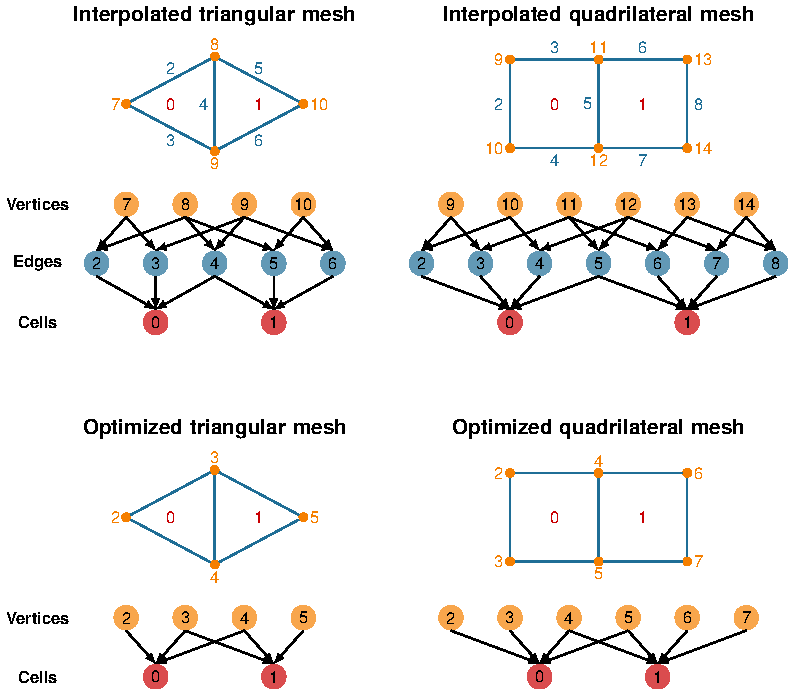
\includegraphics[height=7.3cm]{figs/meshtopology}
   \end{center}
   
 \end{frame}
 

% ------------------------------------------------------------ SLIDE
\begin{frame}
  \frametitle{Governing Equations}
  \summary{}

  Using numerical quadrature we convert the integrals to sums over the
  cells and quadrature points
  \begin{multline}
    -\sum_\text{vol cells} \sum_\text{quad pts} \sigma_{ij} N^n_{,j} w_q |J_\text{cell}|
    + \sum_\text{surf cells} \sum_\text{quad pts} T_i N^n w_q |J_\text{cell}|\\
    + \sum_\text{vol cells} \sum_\text{quad pts}  f_i N^n w_q |J_\text{cell}|\\
    - \sum_\text{vol cells} \sum_\text{quad pts} \rho \sum_m \ddot{a}^m_i N^m N^n w_q |J_\text{cell}| = \vec{0}    
  \end{multline}

\end{frame}


% ------------------------------------------------------------ SLIDE
\begin{frame}
  \frametitle{Quasi-static Solution}
  \summary{Neglect inertial terms}

  \vfill
  Form system of algebraic equations
  \begin{equation}
    \underline{A} (t) \vec{u}(t) = \vec{b}(t)
  \end{equation}
  where
  \begin{gather}
    A^{nm}_{ij}(t) = \sum_\text{vol cells} \sum_\text{quad pts} 
      \frac{1}{4} C_{ijkl}(t) (N^m_{,l} + N^m_{,k})(N^n_{,j} + N^n_{,i}) w_q |J_\text{cell}| \\
    b_i(t) =    
     \sum_\text{surf cells} \sum_\text{quad pts} T_i(t) N^n w_q |J_\text{cell}| 
    + \sum_\text{vol cells} \sum_\text{quad pts}  f_i(t) N^n w_q |J_\text{cell}|
\end{gather}
  and solve for $\vec{u}(t)$.
  \vfill


\end{frame}


% ========================================================== SECTION
\subsection{Fault Implementation}

% ------------------------------------------------------------ SLIDE
\begin{frame}[fragile]
  \frametitle{Fault Interface}
  \summary{Fault tractions couple deformation across interface}

  \begin{center}
    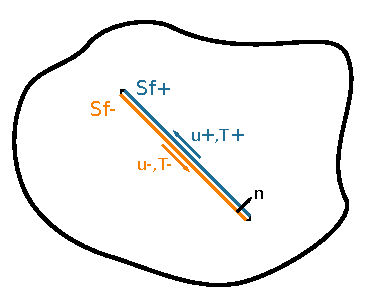
\includegraphics[height=7.0cm]{figs/domaindecomp}
  \end{center}

\end{frame}


% ------------------------------------------------------------ SLIDE
\begin{frame}
  \frametitle{Implementation: Fault Interfaces}
   \summary{Use cohesive cells to control fault behavior}
 
  \begin{center}
    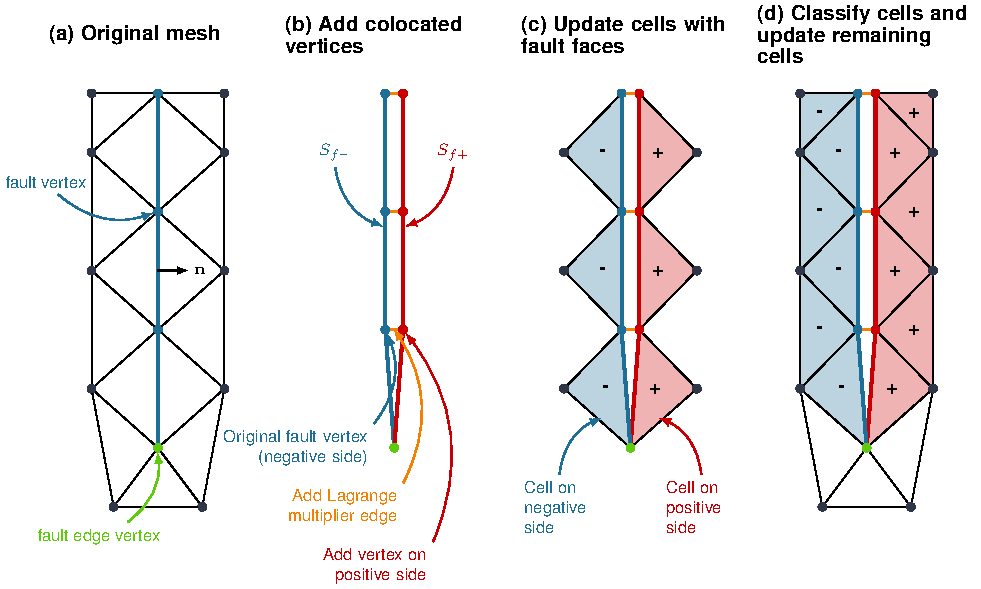
\includegraphics[height=7.0cm]{figs/cohesivecells}
  \end{center}
   
 \end{frame}
 

% ------------------------------------------------------------ SLIDE
\begin{frame}[fragile]
  \frametitle{Fault Implementation: Governing Equations}
  \summary{Terms in governing equation associated with fault}

  \begin{itemize}
  \item Tractions on fault surface are analogous to boundary tractions
    \tikz{
      \matrix [matrix of nodes, ampersand replacement=\&] {
      \node {$ \displaystyle \ldots $}; \&
      \node [below delimiter=\}] {$ \displaystyle + \int_{S_T} \vec{\phi} \cdot \vec{T} \, dS$}; \&
      \node [below delimiter=\}] {$ \displaystyle - \int_{S_{f^+}} \vec{\phi} \cdot \vec{l} \, dS$}; \&
      \node [below delimiter=\}] {$ \displaystyle + \int_{S_{f^-}} \vec{\phi} \cdot \vec{l} \, dS$}; \&
      \ldots = 0 \\
      \& \node {Neumann BC}; \& 
      \node {Fault +}; \&
      \node {Fault -}; \& \\
    };
}
  \item Constraint equation relates slip to relative displacement
    \tikz{
      \matrix [matrix of nodes, ampersand replacement=\&] {
        \node {$ \displaystyle \int_{S_f} \vec{\phi} \cdot ($}; \&
        \node [below delimiter=\}] {$\displaystyle\vec{d}$}; \&
        \node {$ \displaystyle - $}; \&
        \node [below delimiter=\}] {$ \displaystyle (\vec{u}_{+} - \vec{u}_{-}) $}; \&
        \node {$ \displaystyle ) dS = 0 $}; \\
        \& Slip \& \& Relative Disp. \& \\
    };
}
  \end{itemize}

\end{frame}


% ------------------------------------------------------------ SLIDE
\begin{frame}
  \frametitle{Fault Slip Implementation}
  \summary{Use Lagrange multipliers to specify slip}

  \begin{itemize}
  \item System without cohesive cells
    \begin{itemize}
    \item Conventional finite-element elasticity formulation
      \begin{equation}
        \underbar{A} \vec{u} = \vec{b} \nonumber
      \end{equation}
    \item Fault slip associated with relative displacements across fault
      \begin{equation}
        \underbar{C} \vec{u} = \vec{d} \nonumber
      \end{equation}
    \end{itemize}
  \item System with Lagrange multiplier constraints for fault slip
    \begin{equation}
      \left( \begin{array}{cc}
          \underbar{A} & \underbar{C}^T\\
          \underbar{C} & 0
        \end{array} \right)
      \left( \begin{array}{c}
          \vec{u}\\
          \vec{l}
        \end{array}\right)
      =
      \left( \begin{array}{c}
          \vec{b}\\
          \vec{d}
        \end{array} \right)
      \nonumber
    \end{equation}
  \item Prescribed (kinematic) slip\\
    Specify fault slip ($\vec{d}$) and solve for Lagrange multipliers ($\vec{l}$)
  \item Spontaneous (dynamic) slip\\
    Adjust fault slip to be compatible with fault constitutive model
\end{itemize}
  
\end{frame}


% ------------------------------------------------------------ SLIDE
\begin{frame}
  \frametitle{Implementing Fault Slip with Lagrange multipliers}
 
 \begin{itemize}
 \item Advantages
   \begin{itemize}
   \item Fault implementation is local to cohesive cell
   \item Solution includes tractions generating slip (Lagrange multipliers)
   \item Retains block structure of matrix, including symmetry
   \item Offsets in mesh mimic slip on natural faults
   \end{itemize}
 \item Disadvantages 
   \begin{itemize}
   \item Cohesive cells require adjusting topology of finite-element
     mesh
   \item Scalable preconditioner/solver is more complex
  \end{itemize}
 \end{itemize}
  
\end{frame}


% ========================================================== SECTION
\subsection{Running PyLith}

% ------------------------------------------------------------ SLIDE
\begin{frame}
  \frametitle{Workflow for Running PyLith}

  \begin{center}
    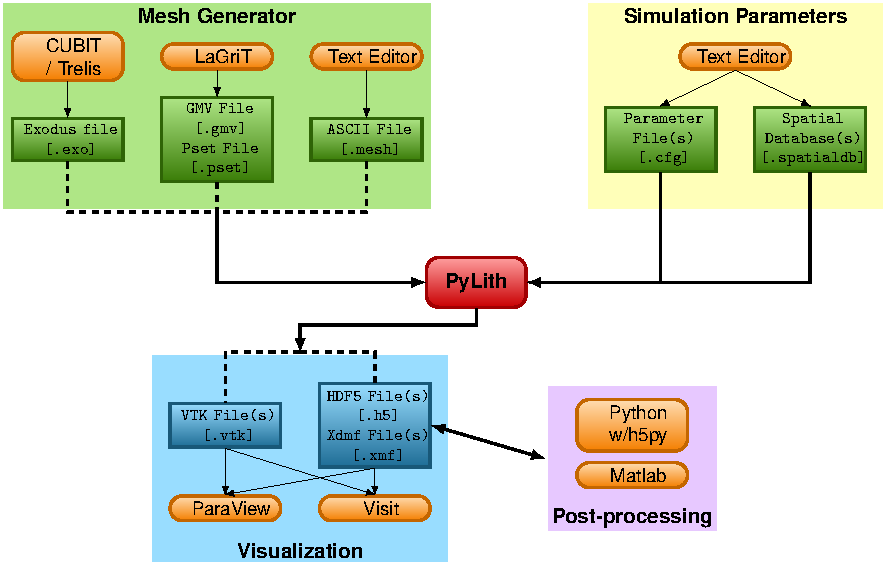
\includegraphics[height=7.2cm]{figs/runpylith}
  \end{center}
   
\end{frame}


% ------------------------------------------------------------ SLIDE
\begin{frame}
  \frametitle{Spatial Databases}
  \summary{User-specified field/value in space}

  \begin{itemize}
 \item Examples
    \begin{itemize}
    \item Uniform value for Dirichlet (0-D)
    \item Piecewise linear variation in tractions for Neumann BC (1-D)
    \item SCEC CVM-H seismic velocity model (3-D)
    \end{itemize}
  \item Generally independent of discretization for problem
  \item Available spatial databases
    \begin{description}
    \item[UniformDB] Optimized for uniform value
    \item[SimpleDB] Simple ASCII files (0-D, 1-D, 2-D, or 3-D)
    \item[SCECCVMH] SCEC CVM-H seismic velocity model v5.3
    \item[ZeroDispDB] Special case of UniformDB
    \end{description}
 \end{itemize}

\end{frame}


% ========================================================== SECTION
\subsection{Features}

% ------------------------------------------------------------ SLIDE
\begin{frame}
  \frametitle{Features in PyLith 2.0}
  \summary{Complete rewrite of finite-element data structures}

  \begin{itemize}
  \item Time integration schemes and elasticity formulations
    \begin{itemize}
    \item Implicit for quasistatic problems (neglect inertial terms)
      \begin{itemize}
      \item Infinitesimal strains
      \item Small strains
      \end{itemize}
    \item Explicit for dynamic problems
      \begin{itemize}
      \item Infinitesimal strains
      \item Small strains
      \item Numerical damping via viscosity
     \end{itemize}
    \end{itemize}
  \item Bulk constitutive models (2-D, and 3-D)
    \begin{itemize}
    \item Elastic model 
    \item Linear Maxwell viscoelastic models
    \item Generalized Maxwell viscoelastic models
    \item Power-law viscoelastic model
    \item Drucker-Prager elastoplastic model
    \end{itemize}
 \end{itemize}

\end{frame}


% ------------------------------------------------------------ SLIDE
\begin{frame}
  \frametitle{Features in PyLith 2.0 (cont.)}
  \summary{}

  \begin{itemize}
  \item Boundary and interface conditions
    \begin{itemize}
    \item Time-dependent Dirichlet boundary conditions
    \item Time-dependent Neumann (traction) boundary conditions
    \item Absorbing boundary conditions
    \item Kinematic (prescribed slip) fault interfaces w/multiple ruptures
    \item Dynamic (friction) fault interfaces
    \item Time-dependent point forces
    \item Gravitational body forces
    \end{itemize}
  \item Fault constitutive models
    \begin{itemize}
    \item Static friction
    \item Linear slip-weakening
    \item Linear time-weakening
    \item Dieterich-Ruina rate and state friction w/ageing law
   \end{itemize}
 \end{itemize}

\end{frame}


% ------------------------------------------------------------ SLIDE
\begin{frame}
  \frametitle{Features in PyLith 2.0 (cont.)}
  \summary{}

  \begin{itemize}
  \item Automatic and user-controlled time stepping
  \item Ability to specify initial stress/strain state
  \item Importing meshes
    \begin{itemize}
    \item LaGriT: GMV/Pset
    \item CUBIT: Exodus II
    \item ASCII: PyLith mesh ASCII format (intended for toy problems only)
    \end{itemize}
  \item Output: VTK and HDF5 files
    \begin{itemize}
    \item Solution over volume
    \item Solution over surface boundary
    \item Solution interpolated to user-specified points
    \item State variables (e.g., stress and strain) for each material
    \item Fault information (e.g., slip and tractions)
    \end{itemize}
  \item Automatic conversion of units for all parameters
  \item Parallel uniform global refinement
  \item PETSc linear and nonlinear solvers
    \begin{itemize}
    \item Custom preconditioner with algebraic multigrid solver
    \end{itemize}
 \end{itemize}
  
\end{frame}


% ------------------------------------------------------------ SLIDE
\begin{frame}
  \frametitle{PyLith Development}
  \summary{See PyLith User Resources for detailed development plan}

  \begin{itemize}
  \item Immediate priorities \status{in progress}
    \begin{itemize}
    \item New fault implementation for spontaneous rupture\\
      Much faster convergence for quasi-static simulations
    \item Improved handling of fault intersections
    \end{itemize}
  \item Short-term priorities
    \begin{itemize}
    \item Under-the-hood improvements
      \begin{itemize}
      \item Support higher order basis functions \status{in
          progress}\\
        Provides much higher resolution for a given mesh
      \item Multigrid nonlinear solver \status{in progress}
      \item Prepare for multi-physics
      \end{itemize}
    \item Multi-cycle earthquake modeling\\
      Resolve interseismic, coseismic, and postseismic deformation
      \begin{itemize}
      \item Coupling solvers for quasistatic and dynamic deformation
      \item Adaptive time stepping
      \end{itemize}
    \item Multiphysics: Elasticity + Fluid flow + Heat flow
    \item Scaling to 1000 cores
    \end{itemize}
  \end{itemize}

\end{frame}


% ------------------------------------------------------------ SLIDE
\begin{frame}
  \frametitle{PyLith Development}
  \summary{Planned Releases}

  \begin{itemize}
  \item v2.1 (Summer 2014)
    \begin{itemize}
    \item New fault implementation for spontaneous rupture
    \item Improved handling of fault intersections
    \end{itemize}
  \item v3.0 (Early 2015)
    \begin{itemize}
    \item Support for higher order basis functions
    \item Adaptive time stepping
    \end{itemize}
  \item v3.1 (Mid-Late 2015)
    \begin{itemize}
    \item Support for incompressible elasticity
    \item Heat and fluid flow coupled to elastic deformation
    \end{itemize}
  \end{itemize}

\end{frame}


% ========================================================== SECTION
\subsection{Architecture}

% ------------------------------------------------------------ SLIDE
\begin{frame}
  \frametitle{Design Philosophy}
  \summary{Modular, extensible, and smart}

  \begin{itemize}
  \item Code should be flexible and modular
  \item Users should be able to add new features without modifying
    code, for example:
    \begin{itemize}
    \item Boundary conditions
    \item Bulk constitutive models
    \item Fault constitutive models
    \end{itemize}
  \item Input/output should be user-friendly
  \item Top-level code written in Python (expressive, dynamic typing)
  \item Low-level code written in C++ (modular, fast)
\end{itemize}

\end{frame}


% ------------------------------------------------------------ SLIDE
\begin{frame}
  \frametitle{PyLith Design: Focus on Geodynamics}
  \summary{Leverage packages developed by computational scientists}

  \documentclass[tikz, border=2pt]{standalone}
\usepackage[none]{hyphenat}
\usepackage{helvet}
\renewcommand{\familydefault}{phv}

\makeatletter
\renewcommand{\normalsize}{\@setfontsize\normalsize{6}{6.5}}
\makeatother

\usepackage{tikz}

\begin{document}
\pagestyle{empty}

\definecolor{yellow}{rgb}{1.0, 1.0, 0.45} % 255/255/115
\definecolor{dkyellow}{rgb}{0.9, 0.9, 0.0} % % 230/230/0

\definecolor{ltorange}{rgb}{1.0, 0.74, 0.41} % 255/188/105
\definecolor{orange}{rgb}{0.96, 0.50, 0.0} % 246/127/0

\definecolor{ltred}{rgb}{1.0, 0.25, 0.25} % 255/64/64
\definecolor{red}{rgb}{0.79, 0.00, 0.01} % 201/0/3

\definecolor{ltpurple}{rgb}{0.81, 0.57, 1.00} % 206/145/255
\definecolor{purple}{rgb}{0.38, 0.00, 0.68} % 97/1/175

\definecolor{ltblue}{rgb}{0.2, 0.73, 1.0} % 51/187/255
\definecolor{blue}{rgb}{0.12, 0.43, 0.59} % 30/110/150

\definecolor{ltltgreen}{rgb}{0.7, 1.00, 0.7} % 96/204/14
\definecolor{ltgreen}{rgb}{0.37, 0.80, 0.05} % 96/204/14
\definecolor{green}{rgb}{0.23, 0.49, 0.03} % 59/125/8
  
\definecolor{dkslate}{rgb}{0.18, 0.21, 0.28} % 47/53/72
\definecolor{mdslate}{rgb}{0.45, 0.50, 0.68} % 114/127/173
\definecolor{ltslate}{rgb}{0.85, 0.88, 0.95} % 216/225/229


\usetikzlibrary{arrows,shapes}
\usetikzlibrary{shadows.blur}

\tikzstyle{generic} = [
  rectangle,
  text centered,
  rounded corners=0.75em,
  minimum width=5em, 
  minimum height=2.0em,
  blur shadow={shadow blur steps=5}]

\tikzstyle{level0} = [generic, 
                      draw=ltblue!80!black,
                      top color=ltblue!50!white,
                      bottom color=ltblue,]
\tikzstyle{level1} = [generic, 
                      draw=ltgreen!80!black,
                      top color=ltgreen!50!white,
                      bottom color=ltgreen]
\tikzstyle{level2} = [generic, 
                      draw=orange!80!black,
                      top color=ltorange!50!white,
                      bottom color=orange]
\tikzstyle{level3} = [generic, 
                      draw=ltred!80!black,
                      top color=ltred!50!white,
                      bottom color=ltred]

\tikzstyle{arrowto} = [->, thick]
\tikzstyle{arrow01} = [arrowto, color=green!80!black]

\tikzstyle{arrow02} = [arrowto, color=orange!80!black]
\tikzstyle{arrow12} = [arrowto, color=orange!80!black]

\tikzstyle{arrow13} = [arrowto, color=red!80!black]
\tikzstyle{arrow23} = [arrowto, color=red!80!black]

\begin{tikzpicture}[
  node distance=6.0em,
  thick]

  % Level 0
  \node (pylith) [level0] {PyLith};

  % Level 1
  \node (spatialdata) [level1, below of=pylith, xshift=+4em, yshift=+1em] {spatialdata};
  \node (petsc) [level1, left of=spatialdata, xshift=-2em] {PETSc};

  \path (pylith) edge[arrow01] (petsc);
  \path (pylith) edge[arrow01] (spatialdata);

  % Level 2
  \node (proj4) [level2, below of=spatialdata, xshift=-2em, yshift=+1em] {Proj.4};
  \node (hdf5) [level2, left of=proj4, xshift=0em] {HDF5};
  \node (netcdf) [level2, left of=hdf5, xshift=-1em] {NetCDF};
  \node (pyre) [level2, right of=proj4, xshift=0em] {Pyre};
  \node (numpy) [level2, right of=pyre, xshift=0em] {numpy};

  \path (petsc) edge[arrow12] (hdf5);
  \path (spatialdata) edge[arrow12] (pyre);
  \path (spatialdata) edge[arrow12] (proj4);
  \path (spatialdata) edge[arrow12] (numpy);
  \path (netcdf) edge[arrow12] (hdf5);

  \path (pylith) edge[arrow02, bend left=15] (hdf5);
  \path (pylith) edge[arrow02, bend right=30] (netcdf);
  \path (pylith) edge[arrow02, bend left=40] (pyre);

  % Level 3
  \node (mpi) [level3, below of=proj4, yshift=+1em] {MPI};
  \node (blas) [level3, left of=mpi, xshift=-4em] {BLAS/LAPACK};

  \path (pyre) edge[arrow23] (mpi);
  \path (hdf5) edge[arrow23] (mpi);

  \path (petsc) edge[arrow13] (mpi);
  \path (petsc) edge[arrow13, bend right=20] (blas);


\end{tikzpicture}

\end{document}


\end{frame}


% ------------------------------------------------------------ SLIDE
\begin{frame}[fragile]
  \frametitle{PyLith Application Flow}
  \summary{}
 
{\small\tt
  \begin{minipage}[t]{2.0in}
      \begin{block}{PyLithApp}
        \begin{verbatim}
main()
  mesher.create()
  problem.initialize()
  problem.run()
\end{verbatim}
    \end{block}
    \begin{block}{TimeDependent (Problem)}
    \begin{verbatim}
initialize()
  formulation.initialize()

run()
  while (t < tEnd)
    dt = formulation.dt()
    formulation.prestep(dt)
    formulation.step(dt)
    formulation.poststep(dt)
\end{verbatim}
  \end{block}
\end{minipage}
  \hfill
  \begin{minipage}[t]{2.0in}
    \begin{block}{Implicit (Formulation)}
      \begin{verbatim}
initialize()

prestep()
  set values of constraints

step()
  compute residual
  solve for disp. incr.

poststep()
   update disp. field
   write output
\end{verbatim}
    \end{block}
  \end{minipage}
}

\end{frame}


% ------------------------------------------------------------ SLIDE
\begin{frame}
  \frametitle{PyLith as a Hierarchy of Components}
  \summary{Components are the basic building blocks}

  \vfill
  \begin{center}
    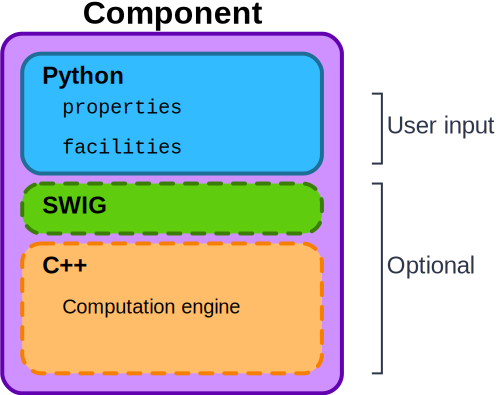
\includegraphics[height=2.0in]{figs/component}
  \end{center}  
  \vfill

\end{frame}


% ------------------------------------------------------------ SLIDE
\begin{frame}
  \frametitle{PyLith as a Hierarchy of Components}
  \summary{PyLith Application and Time-Dependent Problem}

  \vfill
  \begin{center}
    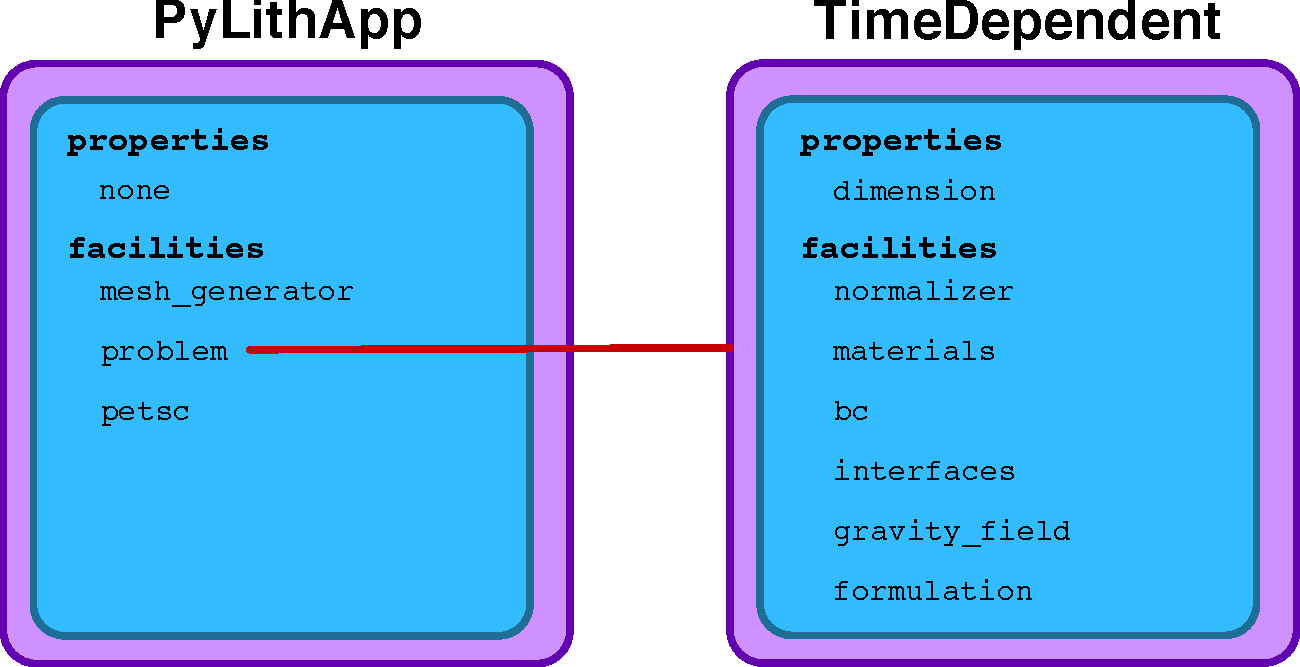
\includegraphics[height=2.0in]{figs/pylithapp}
  \end{center}  
  \vfill

\end{frame}


% ------------------------------------------------------------ SLIDE
\begin{frame}
  \frametitle{PyLith as a Hierarchy of Components}
  \summary{Fault with kinematic (prescribed slip) earthquake rupture}

  \vfill
  \begin{center}
    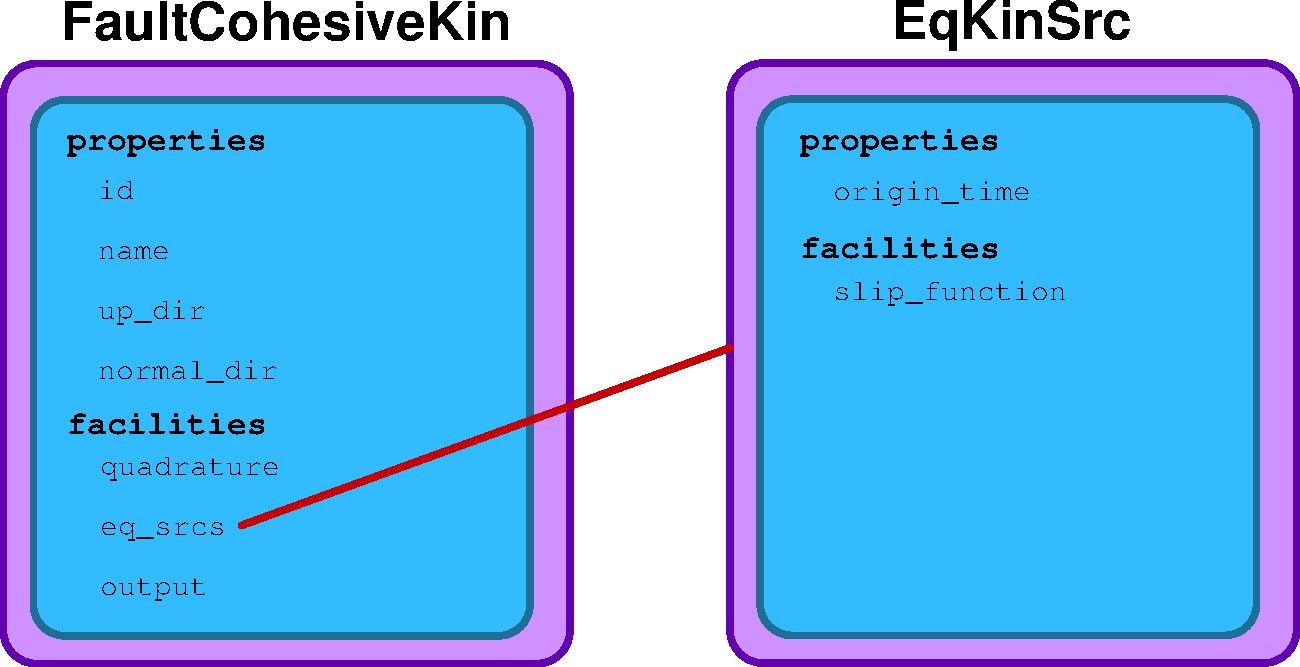
\includegraphics[height=2.0in]{figs/faultcohesivekin}
  \end{center}  
  \vfill

\end{frame}


% ------------------------------------------------------------ SLIDE
\begin{frame}
  \frametitle{PyLith as a Hierarchy of Components}
  \summary{Diagram of simple toy problem}

  \vfill
  \begin{center}
    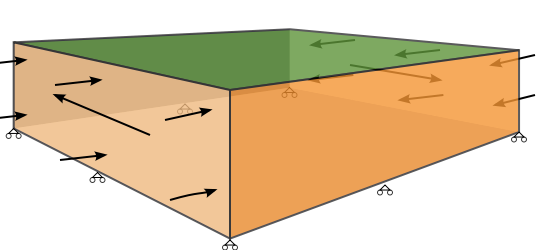
\includegraphics[height=2.0in]{figs/step01_diagram}
  \end{center}  
  \vfill

\end{frame}


% ------------------------------------------------------------ SLIDE
\begin{frame}
  \frametitle{PyLith as a Hierarchy of Components}
  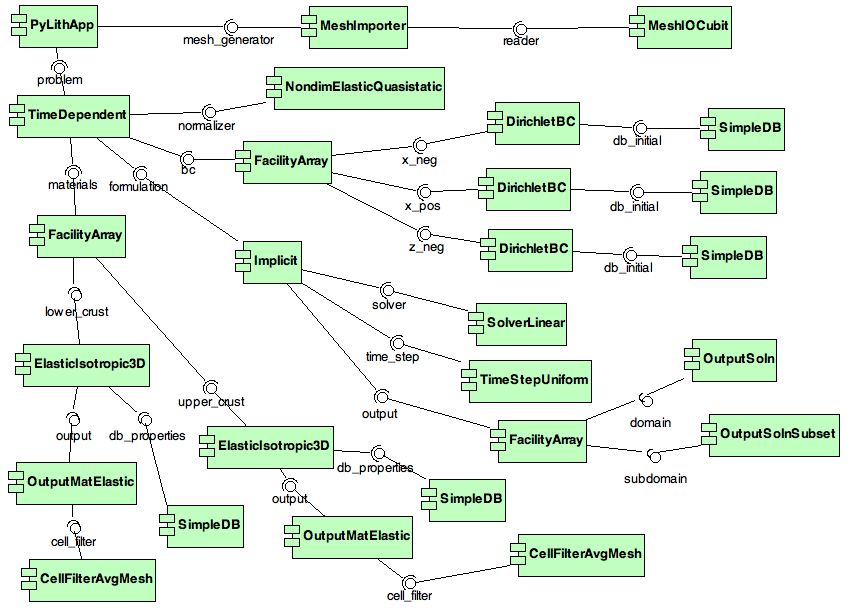
\includegraphics[height=3.2in]{figs/step01_components}
\end{frame}



% ========================================================== SECTION
\subsection{Testing}

% ------------------------------------------------------------ SLIDE
\begin{frame}
  \frametitle{Unit and Regression Testing}
  \summary{Automatically run more than 1800 tests on multiple
    platforms whenever code is checked into the source repository.}

  \begin{itemize}
  \item Create tests for nearly every function in code during development
    \begin{itemize}
    \item Remove most bugs during initial implementation
    \item Isolate and expose bugs at origin
    \end{itemize}
  \item Create new tests to expose reported bugs
    \begin{itemize}
    \item Prevent bugs from reoccurring
    \end{itemize}
  \item Rerun tests whenever code is changed
    \begin{itemize}
    \item Code continually improves (permits optimization with
      quality control)
    \end{itemize}
  \item Binary packages generated automatically upon successful
    completion of tests
  \item Additional full-scale parallel regression tests are run before releases
  \end{itemize}

\end{frame}

% ========================================================== SECTION
\section{CUBIT/Trelis}
\subsection{General}

% ------------------------------------------------------------ SLIDE
\begin{frame}
  \frametitle{Mesh Generation Tips}
  \summary{There is no silver bullet in finite-element mesh generation}
 
  \begin{itemize}
  \item Hex/Quad versus Tet/Tri
    \begin{itemize}
    \item Hex/Quad are slightly more accurate and faster
    \item Tet/Tri easily handle complex geometry
    \item Easy to vary discretization size with Tet, Tri, and Quad cells
    \item There is no easy answer\\
      For a given accuracy, a finer resolution Tet mesh that varies
      the discretization size in a more optimal way {\bf\it might} run
      faster than a Hex mesh
    \end{itemize}
  \item Check and double-check your mesh
    \begin{itemize}
    \item Were there any errors when running the mesher?
    \item Are the boundaries, etc marked correctly for your BC?
    \item Check mesh quality (aspect ratio should be close to 1)
    \end{itemize}
  \end{itemize}

\end{frame}


% ------------------------------------------------------------ SLIDE
\begin{frame}
  \frametitle{CUBIT Workflow}
  \summary{}
 
  \begin{enumerate}
  \item Create geometry
    \begin{enumerate}
    \item Construct surfaces from points, curves, etc or basic shapes
    \item Create domain and subdivide to create any interior surfaces
      \begin{itemize}
      \item Fault surfaces must be interior surfaces (or a subset) that completely divide domain
      \item Need separate volumes for different constitutive {\em models, not parameters}
      \end{itemize}
    \end{enumerate}
  \item Create finite-element mesh
    \begin{enumerate}
    \item Specify meshing scheme
    \item Specify mesh sizing information
    \item Generate mesh
    \item Smooth to fix any poor quality cells
    \end{enumerate}
  \item Create nodesets and blocks
    \begin{enumerate}
    \item Create block for each constitutive model
    \item Create nodeset for each BC and fault
    \item \important{Create nodeset for buried fault edges}
    \item Create nodeset for ground surface for output (optional)
    \end{enumerate}
  \item Export mesh in Exodus II format ({\tt .exo} files)
  \end{enumerate}

\end{frame}


% ------------------------------------------------------------ SLIDE
\begin{frame}
  \frametitle{CUBIT/Trelis Issues}
  \summary{Keep in mind the scales of the observations you are modeling}
 
  \begin{itemize}
  \item Topography/bathymetry
    \begin{itemize}
    \item Ignore topography/bathymetry unless you know it matters
    \item For rectilinear grid, create UV net surface
    \item Convert triangular facets to UV net surface via mapped mesh
    \end{itemize}
  \item Fault surfaces
    \begin{itemize}
    \item Building surfaces from contours is usually easiest
    \item Include features at the resolution that matters
    \end{itemize}
  \item Performance
    \begin{itemize}
    \item Number of points in spline curves/surfaces has huge affect
      on mesh generation runtime
    \item CUBIT/Trelis do not run in parallel
    \item Use uniform global refinement in PyLith for large sims ($>$10M cells) 
    \end{itemize}
  \end{itemize}

\end{frame}


% ------------------------------------------------------------ SLIDE
\begin{frame}
  \frametitle{CUBIT/Trelis Best Practices}
  \summary{}
 
  \begin{description}
    \issue{Changes in geometry cause changes in object ids} {Name objects and use
      APREPRO or Python to eliminate hardwired ids wherever possible}
    \issue{Splines with many points slows down operations}{Reduce the
      number of points per spline}
    \issue{Surfaces meet in small angles creating distorted
      cells}{Trim geometry to eliminate features smaller than cell
      size}
    \issue{Difficulty meshing complex geometry with Hex cells}{Use
      Tet cells even if it requires a finer mesh}
    \issue{Hex mesh over-samples parts of the
      domain}{Use Tet mesh and vary discretization within domain}
    \issue{Extended surfaces create very complex geometry}{Subdivide
      geometry before webcutting to eliminate overly complex geometry}
  \end{description}

\end{frame}


% ========================================================== SECTION
\section{Troubleshooting}
\subsection{General}

% ------------------------------------------------------------ SLIDE
\begin{frame}
  \frametitle{General Numerical Modeling Tips}
  \summary{Start simple and progressively add complexity and increase
    resolution}
  
  \begin{itemize}
  \item \important{Start in 2-D, if possible, and then go to 3-D}
    \begin{itemize}
    \item Much smaller problems $\Rightarrow$ much faster turnaround
    \item Start with an exact solver
    \item Experiment with meshing, boundary conditions, solvers, etc
    \item Keep in mind how physics differs from 3-D
    \end{itemize}
  \item \important{Start with coarse resolution and then increase resolution}
    \begin{itemize}
    \item Much smaller problems $\Rightarrow$ much faster turnaround
    \item Start with an exact solver
    \item Experiment with meshing, boundary conditions, solvers, etc.
    \item Increase resolution until solution resolves features of interest
      \begin{itemize}
      \item Resolution will depend on spatial scales in BC, initial
        conditions, deformation, and geologic structure
      \item Is geometry of domain important? At what resolution?
      \item Displacement field is integral of strains/stresses
      \item Resolving stresses/strains requires fine resolution simulations
      \end{itemize}
    \end{itemize}
  \item \important{Use your intuition and analogous solutions to check
      your results!}
  \end{itemize}
  
\end{frame}


% ========================================================== SECTION
\subsection{PyLith}

% ------------------------------------------------------------ SLIDE
\begin{frame}
  \frametitle{PyLith Tips}
  \summary{}
 
  \begin{itemize}
  \item \important{Read the PyLith User Manual}
  \item \important{Do not ignore error messages and warnings!}
  \item Use an example/benchmark as a starting point
  \item Quasi-static simulations
    \begin{itemize}
    \item Start with a static simulation and then add time dependence
    \item \important{Check that the solution converges at every time step}
    \end{itemize}
  \item Dynamic simulations
    \begin{itemize}
    \item Start with a static simulation
    \item \important{Shortest wavelength seismic waves control cell size}
    \end{itemize}
  \item CIG Short-Term Crustal Dynamics mailing list\\
    {\tt \important{cig-short@geodynamics.org}}
  \item PyLith User Resources\\
    {\small\tt \important{http://wiki.geodynamics.org/software:pylith:start}}
  \end{itemize}

\end{frame}


% ------------------------------------------------------------ SLIDE
\begin{frame}
  \frametitle{PyLith Debugging Tools}
  \summary{}

  \begin{itemize}
  \item {\tt pylithinfo [--verbose] [PyLith args]}\\
    Dumps all parameters with their current values to text file
  \item Command line arguments
    \begin{itemize}
    \item {\tt --help}
    \item {\tt --help-components}
    \item {\tt --help-properties}
    \item {\tt --petsc.start\_in\_debugger} (run in xterm)
    \item {\tt --nodes=N} (to run on N processors on local machine)
    \end{itemize}
  \item Journal info flags turn on writing progress\\
    {\tt [pylithapp.journal.info]}\\
    {\tt timedependent = 1} \\
    \begin{itemize}
    \item Turns on/off info for each type of component independently
    \item Examples turn on writing lots of info to stdout using journal flags
    \end{itemize}
  \end{itemize}

\end{frame}


% ------------------------------------------------------------ SLIDE
\begin{frame}
  \frametitle{Getting Started}
  \summary{}

  \begin{itemize}
  \item Read the PyLith User Manual
  \item Work through the examples
    \begin{itemize}
    \item \important{Chapter 7} of the PyLith manual
    \item Input files are provided with the PyLith binary\\
      {\tt \important{src/pylith-2.0.0/examples}}
    \item Input files are provided with the PyLith source tarball\\
      {\tt \important{src/examples}}
    \end{itemize}
  \item Modify an example to look like a problem of interest
  \end{itemize}

\end{frame}


% ======================================================================
\end{document}


% End of file
